\documentclass[12pt,a4paper]{article}
\usepackage[utf8]{inputenc}
\usepackage[T1]{fontenc}
\usepackage[margin=1in]{geometry}
\usepackage{graphicx}
\usepackage{listings}
\usepackage{xcolor}
\usepackage{booktabs}
\usepackage{enumitem}
\usepackage{fancyhdr}
\usepackage{array}
\usepackage{float}
\usepackage{tikz}
\usetikzlibrary{shapes.geometric, arrows.meta, positioning, fit, calc}
\usepackage{hyperref}

\graphicspath{{TestsScreenshots/}}

\hypersetup{
    colorlinks=true,
    linkcolor=blue!70!black,
    urlcolor=blue!70!black,
    citecolor=blue!70!black
}

\lstdefinestyle{cstyle}{
    language=C,
    basicstyle=\ttfamily\small,
    keywordstyle=\color{blue!80!black}\bfseries,
    commentstyle=\color{gray}\itshape,
    stringstyle=\color{orange!80!black},
    numbers=left,
    numberstyle=\tiny\color{gray},
    numbersep=8pt,
    frame=single,
    framesep=4pt,
    breaklines=true,
    tabsize=4,
    showstringspaces=false,
    backgroundcolor=\color{gray!6}
}

\lstdefinestyle{shellstyle}{
    frame=single,
    backgroundcolor=\color{black!85},
    basicstyle=\ttfamily\small\color{white},
    breaklines=true,
    numbers=none
}

\pagestyle{fancy}
\fancyhf{}
\setlength{\headheight}{14.5pt}
\lhead{ICS 433 -- Operating Systems}
\rhead{Distributed Resource Scheduler}
\rfoot{Page \thepage}

\title{
    \vspace{-0.5cm}
    \textbf{\large ICS 433 -- Operating Systems} \\[0.35cm]
    \textbf{\LARGE Distributed Resource Scheduler} \\[0.25cm]
    \large Final Project Report \\[0.25cm]
    \normalsize King Fahd University of Petroleum \& Minerals
}

\author{
    Rayan Alamri \quad
    Mohammed Alsuhaibani \quad
    Ali Almuzain \quad
    Mohammed Yar
}

\date{May 2026}

\begin{document}
\maketitle
\thispagestyle{fancy}

\begin{center}
\begin{tabular}{>{\bfseries}p{4.2cm}p{3.2cm}p{2.6cm}p{4.2cm}}
\toprule
Student Name & Student ID & Section & Main Contribution \\
\midrule
Rayan Alamri & 202247900 & 51 & Master node, scheduler, queue, worker registry \\
Mohammed Alsuhaibani & 202245800 & 51 & Worker client, executor, FFmpeg workloads \\
Ali Almuzain & 202261580 & 51 & Protocol, serialization, communication layer \\
Mohammed Yar & 202173410 & 51 & ncurses dashboard, UI integration \\
\bottomrule
\end{tabular}
\end{center}

\newpage
\tableofcontents
\newpage

% ==============================================================================
\section{Introduction}

The Distributed Resource Scheduler is a mini operating-system style project implemented in C. It demonstrates how a master node can coordinate a pool of worker nodes across a local network, assign jobs, receive results, monitor worker health, and recover from failures. The project focuses on operating-system concepts rather than high-level frameworks: sockets, threads, process creation, pipes, synchronization, scheduling, worker liveness, and resource-aware execution.

The final version supports multiple workload types, including numerical workloads, parallel matrix chunks, Mandelbrot row chunks, Monte Carlo sampling, and distributed FFmpeg video processing. It also includes a terminal dashboard, Docker-based simulation, task requeueing, heartbeat timeout detection, and performance measurement for one-worker versus three-worker FFmpeg execution.

\section{Problem Statement and Motivation}

Many computers in a lab or local network are underutilized. A single machine can become slow when processing CPU-intensive or media workloads, while other machines remain idle. The goal of this project is to build a small distributed scheduler that can:

\begin{itemize}[noitemsep]
    \item accept jobs from a user or dashboard,
    \item divide selected workloads into independent tasks,
    \item assign tasks to available workers,
    \item collect and aggregate results,
    \item detect worker failure and requeue incomplete work,
    \item display progress and worker status in real time.
\end{itemize}

The motivation is similar to systems such as Hadoop, Kubernetes, or cluster job runners, but implemented at a smaller scale using POSIX primitives. The project therefore provides practical experience with OS-level abstractions while producing a working distributed system.

\section{Complete Working Project}

The final project is a complete working mini distributed scheduler. It includes:

\begin{itemize}[noitemsep]
    \item a master server that accepts workers and submit clients over TCP,
    \item a worker process that registers with the master and executes assigned tasks,
    \item a scheduler with least-loaded selection and round-robin tie breaking,
    \item a thread-safe task queue and worker registry,
    \item fixed-size network messages with byte-order conversion,
    \item fork-based process isolation for workloads,
    \item a live ncurses dashboard,
    \item FFmpeg video splitting, segment processing, merging, and segment cleanup,
    \item heartbeat monitoring with a 15-second stale-worker timeout,
    \item automatic requeueing of unfinished tasks from disconnected or stale workers,
    \item Docker and Docker Compose support for simulation.
\end{itemize}

\section{System Design}

\subsection{High-Level Architecture}

The system follows a master-worker architecture. The master owns global state: task queue, worker registry, scheduler, job summary, and dashboard. Workers are stateless compute nodes from the scheduler's point of view; they receive a task, execute it, and return a result.

\begin{figure}[H]
\centering
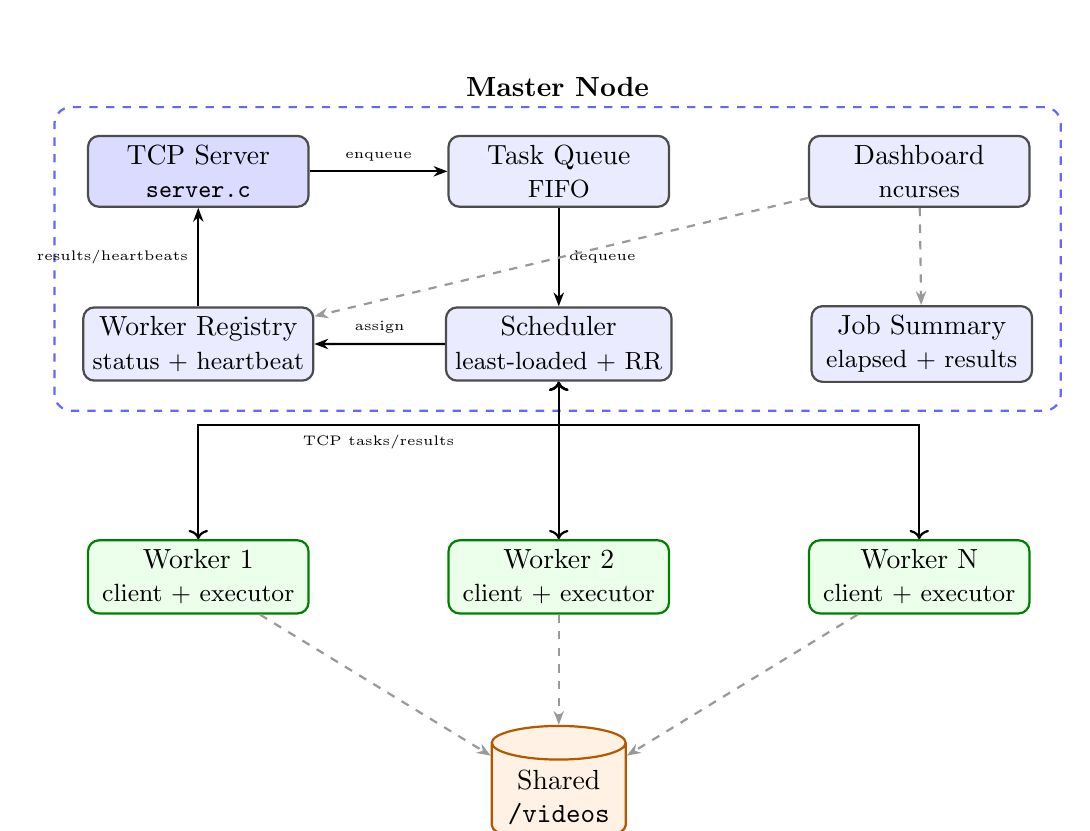
\begin{tikzpicture}[
    node distance=1.25cm and 1.75cm,
    box/.style={rectangle, rounded corners=4pt, draw=black!70, thick,
                minimum width=2.8cm, minimum height=0.9cm,
                align=center, fill=blue!8},
    worker/.style={rectangle, rounded corners=4pt, draw=green!50!black, thick,
                minimum width=2.8cm, minimum height=0.9cm,
                align=center, fill=green!8},
    store/.style={cylinder, shape border rotate=90, aspect=0.28,
                draw=orange!70!black, thick, align=center,
                minimum height=1.1cm, minimum width=1.7cm, fill=orange!10},
    arrow/.style={-{Stealth[length=5pt]}, thick},
    dasharrow/.style={-{Stealth[length=5pt]}, dashed, thick, gray!80}
]

\node[box, fill=blue!14] (server) {TCP Server\\\small\texttt{server.c}};
\node[box, right=of server] (queue) {Task Queue\\\small FIFO};
\node[box, below=of queue] (sched) {Scheduler\\\small least-loaded + RR};
\node[box, below=of server] (registry) {Worker Registry\\\small status + heartbeat};
\node[box, right=of queue] (dash) {Dashboard\\\small ncurses};
\node[box, right=of sched] (job) {Job Summary\\\small elapsed + results};

\node[draw=blue!60, dashed, thick, rounded corners=6pt,
      fit=(server)(queue)(sched)(registry)(dash)(job),
      label=above:\textbf{Master Node},
      inner sep=10pt] (master) {};

\node[worker, below=2.0cm of registry] (w1) {Worker 1\\\small client + executor};
\node[worker, right=of w1] (w2) {Worker 2\\\small client + executor};
\node[worker, right=of w2] (w3) {Worker N\\\small client + executor};
\node[store, below=1.4cm of w2] (videos) {Shared\\\texttt{/videos}};

\draw[arrow] (server) -- node[above, font=\tiny]{enqueue} (queue);
\draw[arrow] (queue) -- node[right, font=\tiny]{dequeue} (sched);
\draw[arrow] (sched) -- node[above, font=\tiny]{assign} (registry);
\draw[dasharrow] (dash) -- (registry);
\draw[dasharrow] (dash) -- (job);
\draw[arrow] (registry) -- node[left, font=\tiny]{results/heartbeats} (server);

\draw[arrow, <->] (sched.south) -- ++(0,-0.55) -| node[pos=0.25, below, font=\tiny]{TCP tasks/results} (w1.north);
\draw[arrow, <->] (sched.south) -- ++(0,-0.55) -| (w2.north);
\draw[arrow, <->] (sched.south) -- ++(0,-0.55) -| (w3.north);
\draw[dasharrow] (w1) -- (videos);
\draw[dasharrow] (w2) -- (videos);
\draw[dasharrow] (w3) -- (videos);

\end{tikzpicture}
\caption{Framework and architecture diagram for the Distributed Resource Scheduler.}
\end{figure}

\subsection{Workflow Diagram}

\begin{figure}[H]
\centering
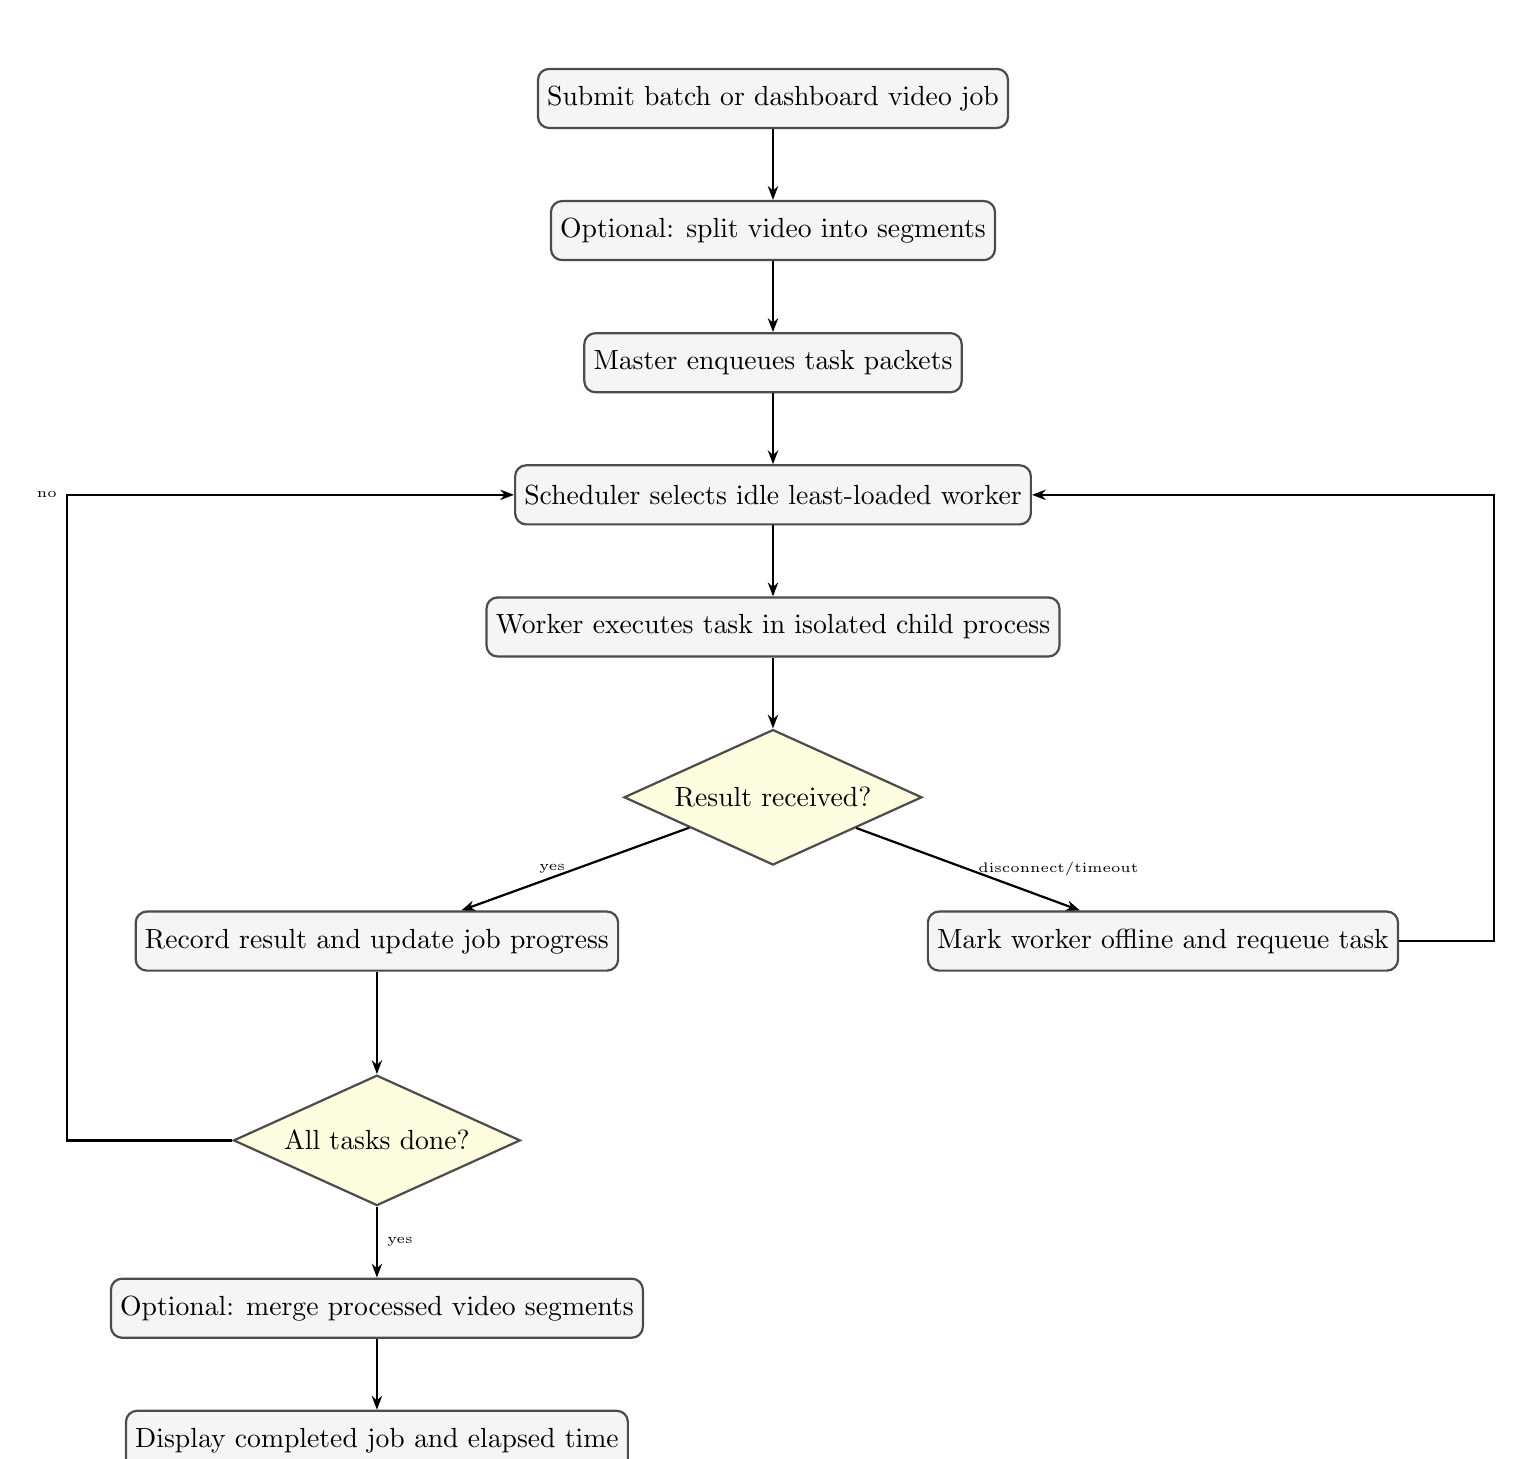
\begin{tikzpicture}[
    node distance=0.9cm,
    flowstep/.style={rectangle, rounded corners=4pt, draw=black!70, thick,
                 minimum width=4.5cm, minimum height=0.75cm,
                 align=center, fill=gray!8},
    decision/.style={diamond, draw=black!70, thick, aspect=2.2,
                 align=center, fill=yellow!12},
    arrow/.style={-{Stealth[length=5pt]}, thick}
]
\node[flowstep] (submit) {Submit batch or dashboard video job};
\node[flowstep, below=of submit] (split) {Optional: split video into segments};
\node[flowstep, below=of split] (queue) {Master enqueues task packets};
\node[flowstep, below=of queue] (schedule) {Scheduler selects idle least-loaded worker};
\node[flowstep, below=of schedule] (worker) {Worker executes task in isolated child process};
\node[decision, below=of worker] (result) {Result received?};
\node[flowstep, below left=1.0cm and 1.0cm of result] (record) {Record result and update job progress};
\node[flowstep, below right=1.0cm and 1.0cm of result] (requeue) {Mark worker offline and requeue task};
\node[decision, below=1.3cm of record] (done) {All tasks done?};
\node[flowstep, below=of done] (merge) {Optional: merge processed video segments};
\node[flowstep, below=of merge] (complete) {Display completed job and elapsed time};

\draw[arrow] (submit) -- (split);
\draw[arrow] (split) -- (queue);
\draw[arrow] (queue) -- (schedule);
\draw[arrow] (schedule) -- (worker);
\draw[arrow] (worker) -- (result);
\draw[arrow] (result) -- node[left, font=\tiny]{yes} (record);
\draw[arrow] (result) -- node[right, font=\tiny]{disconnect/timeout} (requeue);
\draw[arrow] (requeue.east) -- ++(1.2,0) |- (schedule.east);
\draw[arrow] (record) -- (done);
\draw[arrow] (done) -- node[right, font=\tiny]{yes} (merge);
\draw[arrow] (done.west) -- ++(-2.1,0) |- node[left, font=\tiny]{no} (schedule.west);
\draw[arrow] (merge) -- (complete);
\end{tikzpicture}
\caption{End-to-end task workflow, including fault recovery.}
\end{figure}

\subsection{Module Explanation}

\begin{center}
\begin{tabular}{p{3.6cm}p{5.2cm}p{5.2cm}}
\toprule
\textbf{Module} & \textbf{Files} & \textbf{Responsibility} \\
\midrule
Master server & \texttt{src/master/server.c} & TCP accept loop, worker threads, job summaries, dashboard submission API, video pipeline helpers \\
Scheduler and registry & \texttt{src/master/scheduler.c/.h} & Worker table, scheduling algorithm, heartbeat timeout, offline marking \\
Task queue & \texttt{src/master/queue\_mgr.c/.h} & Thread-safe FIFO queue and requeue operations \\
Status API & \texttt{src/master/status.c/.h} & Snapshot generation for dashboard and JSON reporting \\
Worker client & \texttt{src/worker/client.c/.h} & Connects to master, sends heartbeats, receives tasks, sends results \\
Executor & \texttt{src/worker/executor.c/.h} & Forks child processes and runs workloads in isolation \\
Protocol & \texttt{src/shared/protocol.c/.h}, \texttt{models.h} & Fixed-size message frame, byte-order conversion, reliable send/receive \\
Dashboard & \texttt{src/ui/dashboard.c/.h} & ncurses monitoring UI and job submission forms \\
Scripts and Docker & \texttt{Makefile}, \texttt{Dockerfile}, \texttt{docker-compose.yml}, \texttt{scripts/} & Build, simulation, video split/submit/merge helpers \\
\bottomrule
\end{tabular}
\end{center}

\subsection{Project Structure}

The repository is organized by runtime role. The \texttt{src/} directory contains the C implementation, while scripts, Docker files, tests, documentation, and video folders support building, simulation, validation, and FFmpeg workloads.

\begin{lstlisting}[style=shellstyle]
distributed-resource-scheduler/
  README.md                  user-facing overview and run instructions
  MANUAL.md                  extended run and testing manual
  Makefile                   native build, tests, demos, video helpers
  Dockerfile                 container image for master, worker, submit
  docker-compose.yml         compose-based local cluster simulation
  src/
    master/
      server.c/.h            TCP accept loop, worker threads, job API
      scheduler.c/.h         worker registry, assignment, heartbeat timeout
      queue_mgr.c/.h         thread-safe FIFO queue and requeue logic
      status.c/.h            dashboard/JSON snapshots of master state
    worker/
      client.c/.h            worker registration, heartbeats, result sending
      executor.c/.h          fork-isolated workload execution
    client/
      submit.c               command-line task submitter
    shared/
      models.h               message types, worker states, command codes
      protocol.c/.h          reliable socket send/receive and byte order
    ui/
      dashboard.c/.h         ncurses dashboard and built-in submission forms
  scripts/
    split_video.sh           split input videos into segment tasks
    submit_ffmpeg.sh         submit segment tasks from the shell
    merge_video.sh           merge processed video segments
  tests/
    test_scheduler.c         queue, registry, scheduler, protocol tests
    test_worker_executor.c   worker executor and workload tests
  docs/
    Finanl_report/           LaTeX report and report screenshots
  videos/
    input/                   input videos selected by the dashboard
    segments/                generated input segments
    processed/               worker-produced processed segments
    final/                   merged output videos
\end{lstlisting}

\section{Implementation Details}

\subsection{Network Protocol}

All master-worker and submit-master communication uses a fixed-size \texttt{NetworkPayload}. Each field is converted to network byte order before transmission and restored to host byte order after reception. The protocol avoids partial-read bugs by using \texttt{send\_full()} and \texttt{recv\_full()}, which loop until the full payload has been transferred.

\begin{lstlisting}[style=cstyle, caption={Network payload shape.}]
typedef struct {
    uint32_t type;
    uint32_t worker_id;
    uint32_t task_id;
    uint32_t command_code;
    uint32_t argument;
    uint32_t result;
} NetworkPayload;
\end{lstlisting}

\subsection{Scheduling Algorithm}

The final scheduler uses a least-loaded strategy with round-robin tie breaking:

\begin{enumerate}[noitemsep]
    \item dequeue a task from the FIFO queue,
    \item scan for idle workers,
    \item choose the idle worker with the fewest completed tasks,
    \item if several workers are tied, use a rotating round-robin index,
    \item mark the worker busy before sending the task,
    \item on send failure, requeue the task and mark the worker offline.
\end{enumerate}

This balances work better than pure round-robin when workers are heterogeneous. A faster worker can complete more tasks and return to idle sooner, while the tie breaker prevents the same worker from always being selected first.

\subsection{Fault Tolerance}

Fault tolerance is implemented using three mechanisms:

\begin{itemize}[noitemsep]
    \item \textbf{Socket disconnect handling:} if a worker socket closes while it is busy, the master requeues the worker's unfinished task.
    \item \textbf{Send failure handling:} if the scheduler cannot send a task to a selected worker, the task is returned to the queue.
    \item \textbf{Heartbeat timeout:} if no heartbeat arrives for more than 15 seconds, the scheduler marks the worker offline and requeues its current task if one exists.
\end{itemize}

The project intentionally treats disconnected tasks as incomplete rather than failed. A task is marked failed only when a worker returns a workload-specific failure result, such as an FFmpeg timeout or missing segment.

\subsection{Worker Execution and Process Isolation}

Each worker executes tasks through \texttt{executor\_run\_task()}. The executor forks a child process, runs the workload inside that child, writes the result through a pipe, and exits. The parent reads the pipe, waits for the child with \texttt{waitpid()}, and sends the result to the master. This isolates workload crashes from the worker's network state.

\subsection{Supported Workloads}

\begin{center}
\begin{tabular}{clp{7.5cm}}
\toprule
\textbf{Cmd} & \textbf{Name} & \textbf{Description} \\
\midrule
1 & \texttt{prime} & Count primes up to an upper bound. \\
2 & \texttt{matrix} & Compute checksum of one full virtual matrix. \\
3 & \texttt{prime\_range} & Parallel prime counting over independent ranges. \\
4 & \texttt{monte\_carlo} & Parallel Monte Carlo sampling for estimating pi. \\
5 & \texttt{mandelbrot} & Parallel row-chunk checksum for Mandelbrot rows. \\
6 & \texttt{ffmpeg\_segment} & Parallel FFmpeg processing of video segments. \\
7 & \texttt{ffmpeg\_script} & Parallel custom FFmpeg script execution per segment. \\
8 & \texttt{matrix\_parallel} & Parallel matrix checksum using 100-row chunks. \\
\bottomrule
\end{tabular}
\end{center}

\subsection{FFmpeg Video Pipeline}

For video workloads, the master or helper scripts split an input video into files such as \texttt{part\_000.mp4}, \texttt{part\_001.mp4}, and so on. Each segment becomes a separate task. Workers process segments into \texttt{videos/processed/}, and the master merges processed segments into \texttt{videos/final/}. After a segment is successfully processed, its original input segment is deleted because it is no longer needed.

\subsection{Tools and Technologies}

\begin{itemize}[noitemsep]
    \item C language with POSIX APIs
    \item TCP sockets
    \item pthreads
    \item fork, pipe, waitpid, exec-style process management
    \item ncurses dashboard
    \item FFmpeg and ffprobe
    \item Docker and Docker Compose
    \item GNU Make
    \item LaTeX for documentation
\end{itemize}

\section{Results and Testing}

\subsection{Test Cases}

\begin{center}
\begin{tabular}{p{4.4cm}p{8.7cm}}
\toprule
\textbf{Test} & \textbf{Purpose} \\
\midrule
Queue FIFO test & Verifies tasks leave the queue in submission order. \\
Queue requeue test & Verifies orphaned tasks can be placed back into the queue. \\
Registry tests & Verifies worker add, idle selection, busy exclusion, and offline marking. \\
Protocol roundtrip & Verifies network byte-order conversion preserves all fields. \\
Prime executor test & Verifies prime workload correctness. \\
Matrix executor test & Verifies full matrix checksum correctness. \\
Matrix parallel test & Verifies matrix chunk checksum matches the full matrix result for a small matrix. \\
Monte Carlo test & Verifies sampling result is within an acceptable range. \\
Mandelbrot test & Verifies deterministic row-chunk checksum behavior. \\
FFmpeg integration & Verifies segment processing, merge, output file generation, and segment cleanup. \\
Fault tolerance & Verifies task requeue when a worker disconnects or times out. \\
\bottomrule
\end{tabular}
\end{center}

\subsection{User Interface Screenshots}

The dashboard user interface is divided into four main live areas. The \textbf{Overview} panel summarizes queue length, worker counts, current job state, task completion, failures, and the progress bar. The \textbf{Workers} panel lists each worker ID, state, current task, command, argument, completed-task count, average runtime, current run time, and heartbeat age. The \textbf{Job} panel shows the active or most recent job, including command type, expected tasks, elapsed time, result sum, and argument sum. The \textbf{Activity} panel records recent events such as completed jobs, output video paths, offline workers, and requeued tasks.

\begin{figure}[H]
\centering
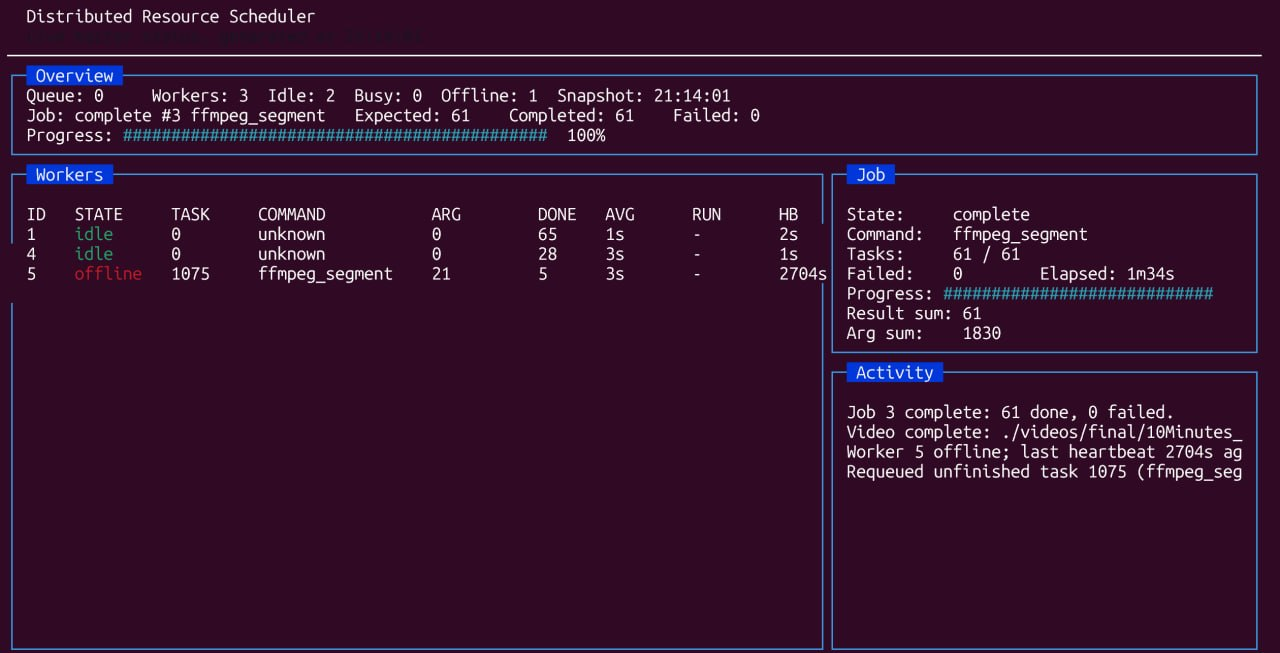
\includegraphics[width=0.95\textwidth]{UI.jpg}
\caption{Main dashboard view showing the Overview, Workers, Job, and Activity panels after an FFmpeg segment job completed.}
\end{figure}

The task submission dialog provides dashboard-side job creation without using the command-line submit client. It exposes the command code, task count, first argument, argument step, range end, and starting task ID. The summary area previews the generated batch and ID range before submission, while the footer shows the available keyboard actions.

\begin{figure}[H]
\centering
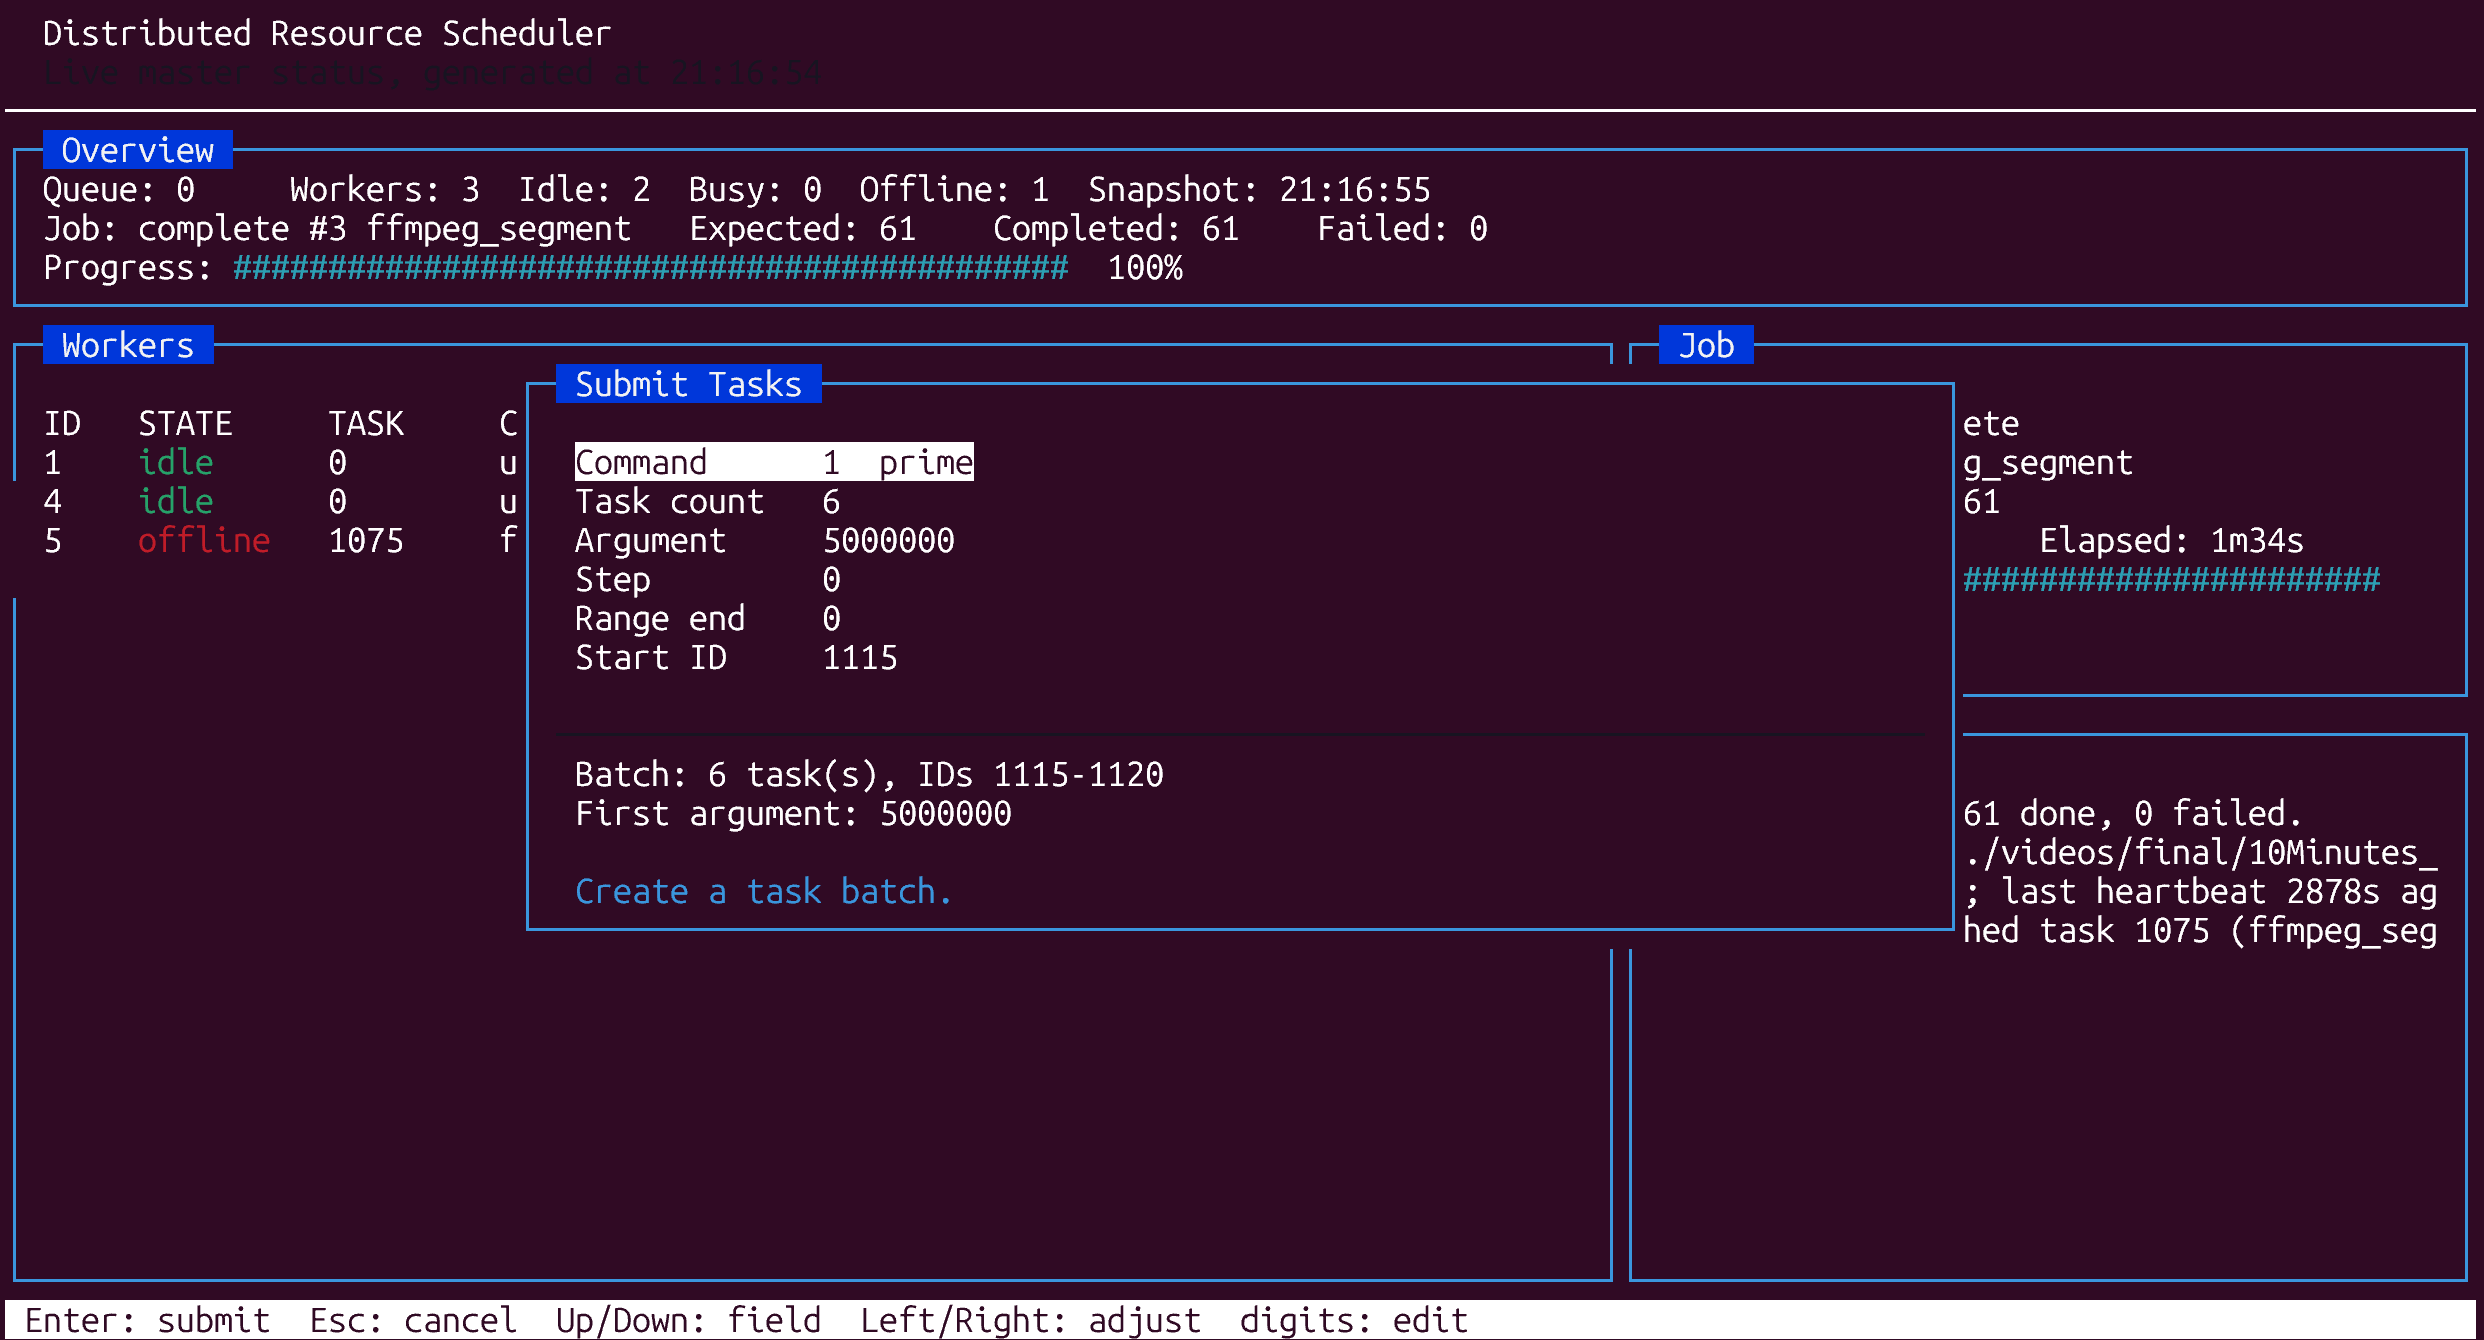
\includegraphics[width=0.95\textwidth]{UI_submitTasks.png}
\caption{Submit Tasks dialog for creating a compute batch directly from the ncurses dashboard.}
\end{figure}

The video processing dialog is specialized for FFmpeg workflows. It lets the user choose an input video, set the segment duration, and select the starting task ID. The dashboard then splits the video, queues one \texttt{ffmpeg\_segment} task per segment, tracks progress through the job panel, and merges the processed segments after the job completes.

\begin{figure}[H]
\centering
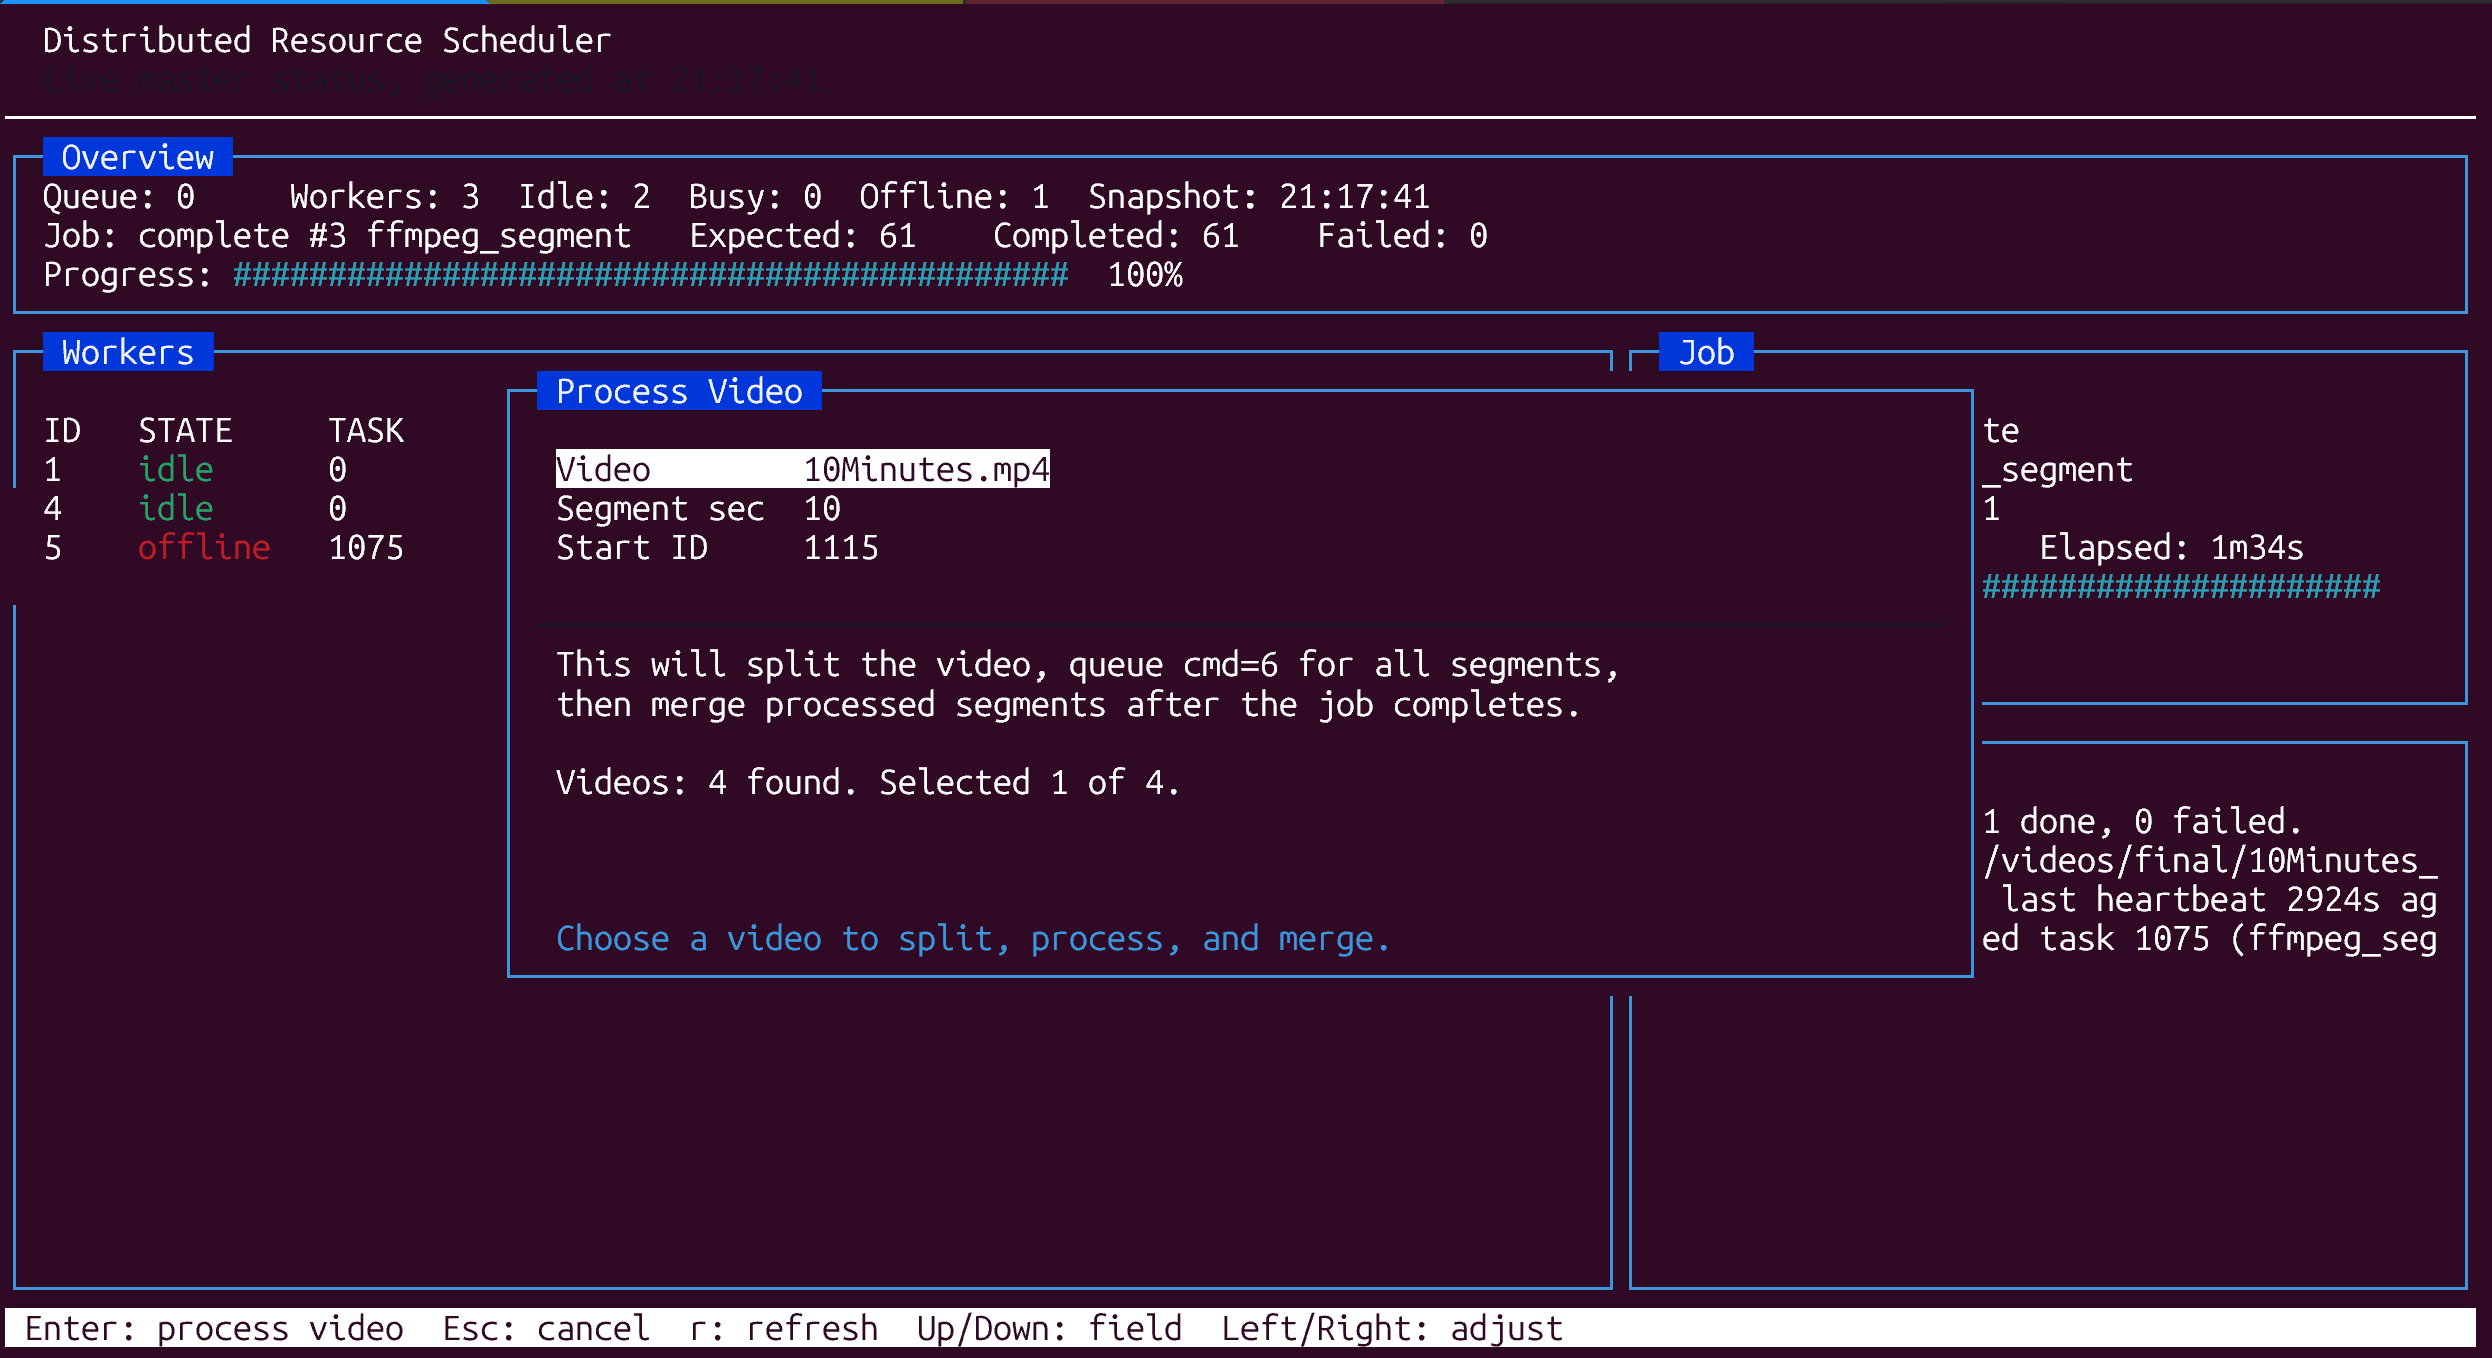
\includegraphics[width=0.95\textwidth]{UI_VideoProcessing.png}
\caption{Process Video dialog used to select an input video and configure distributed segment processing.}
\end{figure}

\subsection{Testing Screenshots}

The following screenshots document the testing evidence for fault tolerance, performance comparison, and unit-test execution.

\begin{figure}[H]
\centering
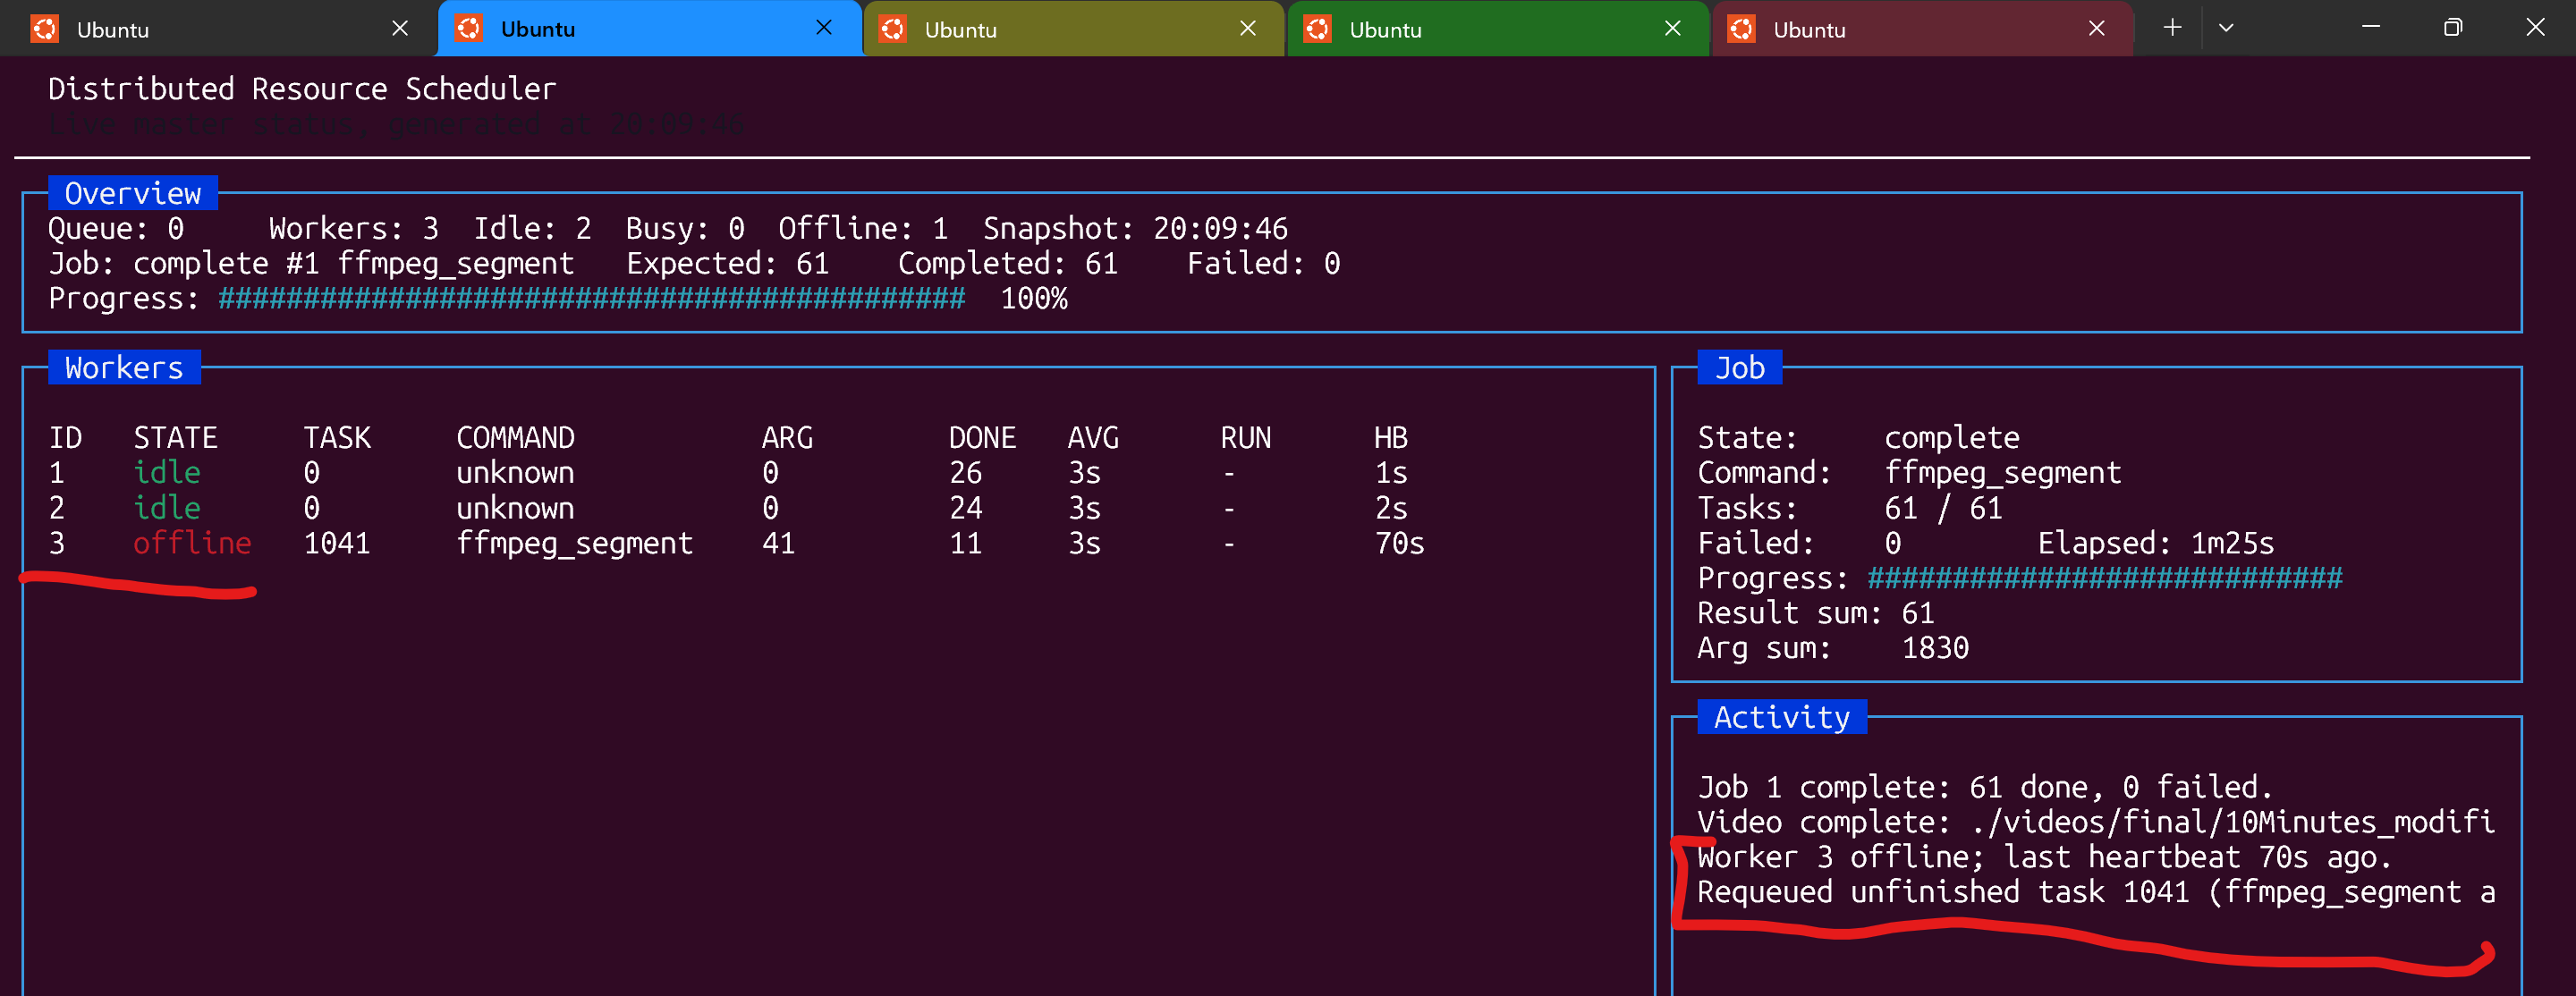
\includegraphics[width=0.95\textwidth]{WorkerFaultTolerance.png}
\caption{Fault tolerance test: a worker is offline and the dashboard reports the unfinished task that was requeued.}
\end{figure}

\begin{figure}[H]
\centering
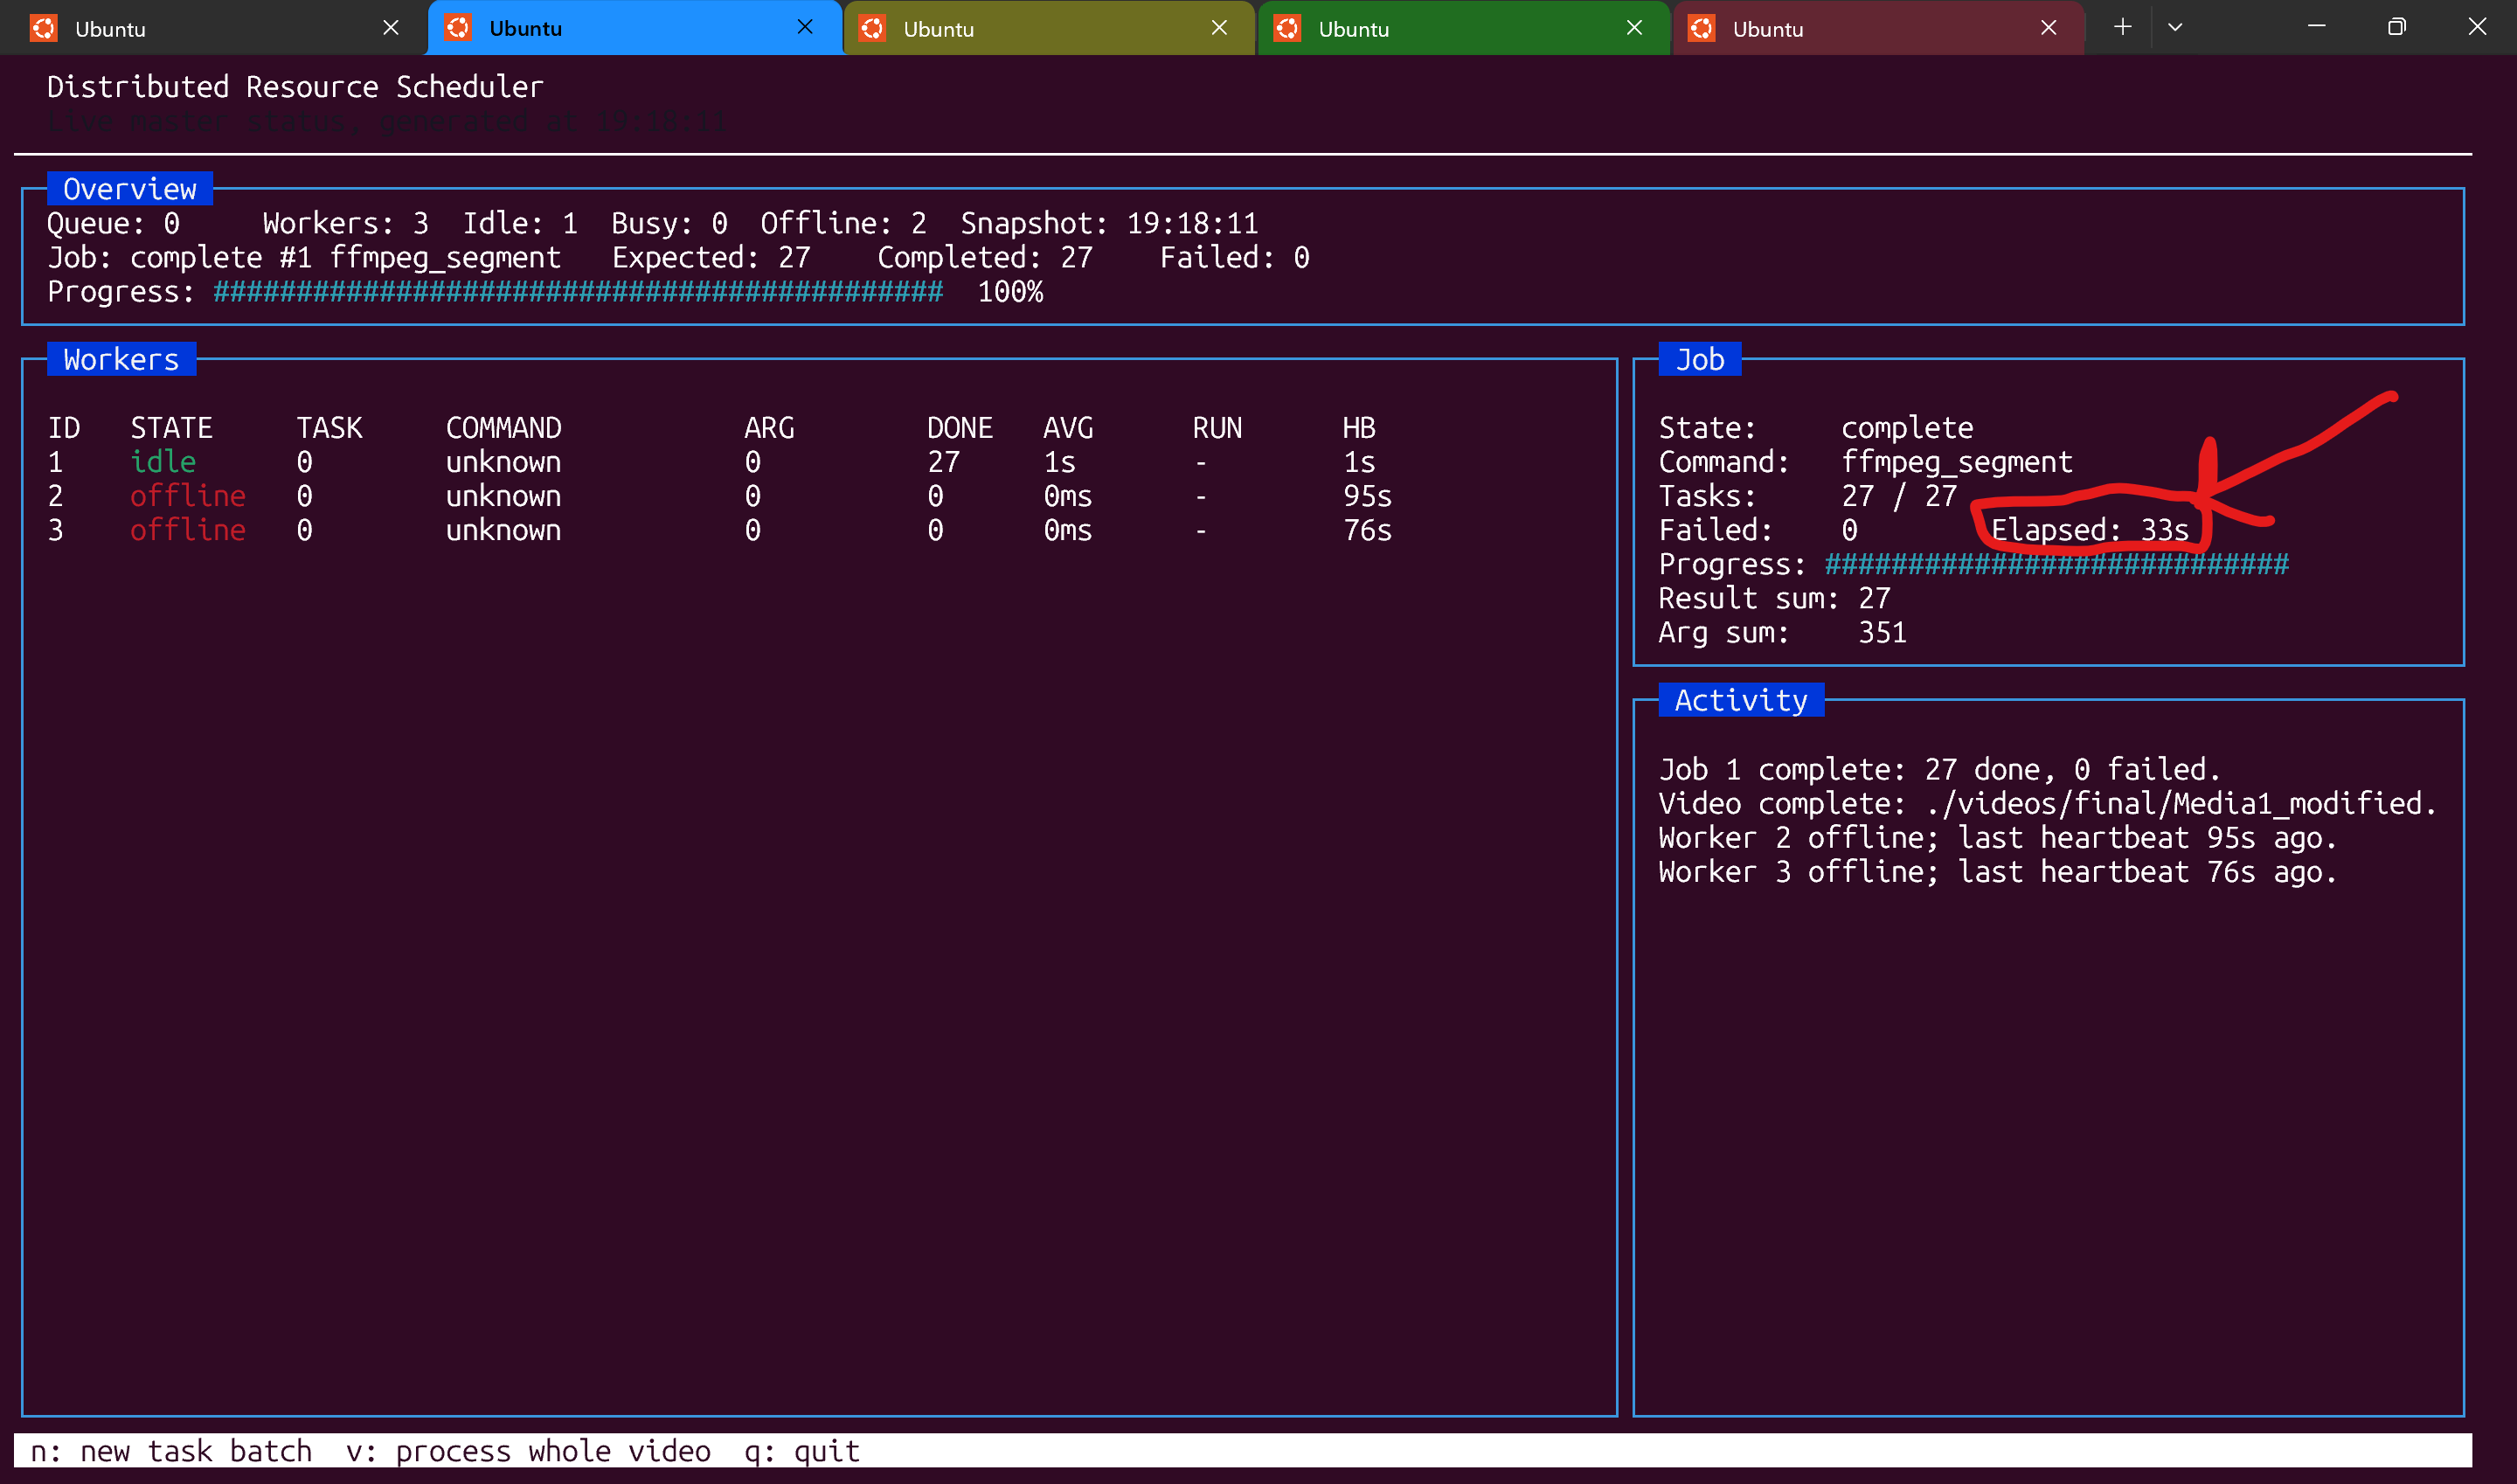
\includegraphics[width=0.95\textwidth]{performance_ffmpeg_using_one_worker.png}
\caption{FFmpeg performance run using one active worker. The dashboard shows the completed job elapsed time.}
\end{figure}

\begin{figure}[H]
\centering
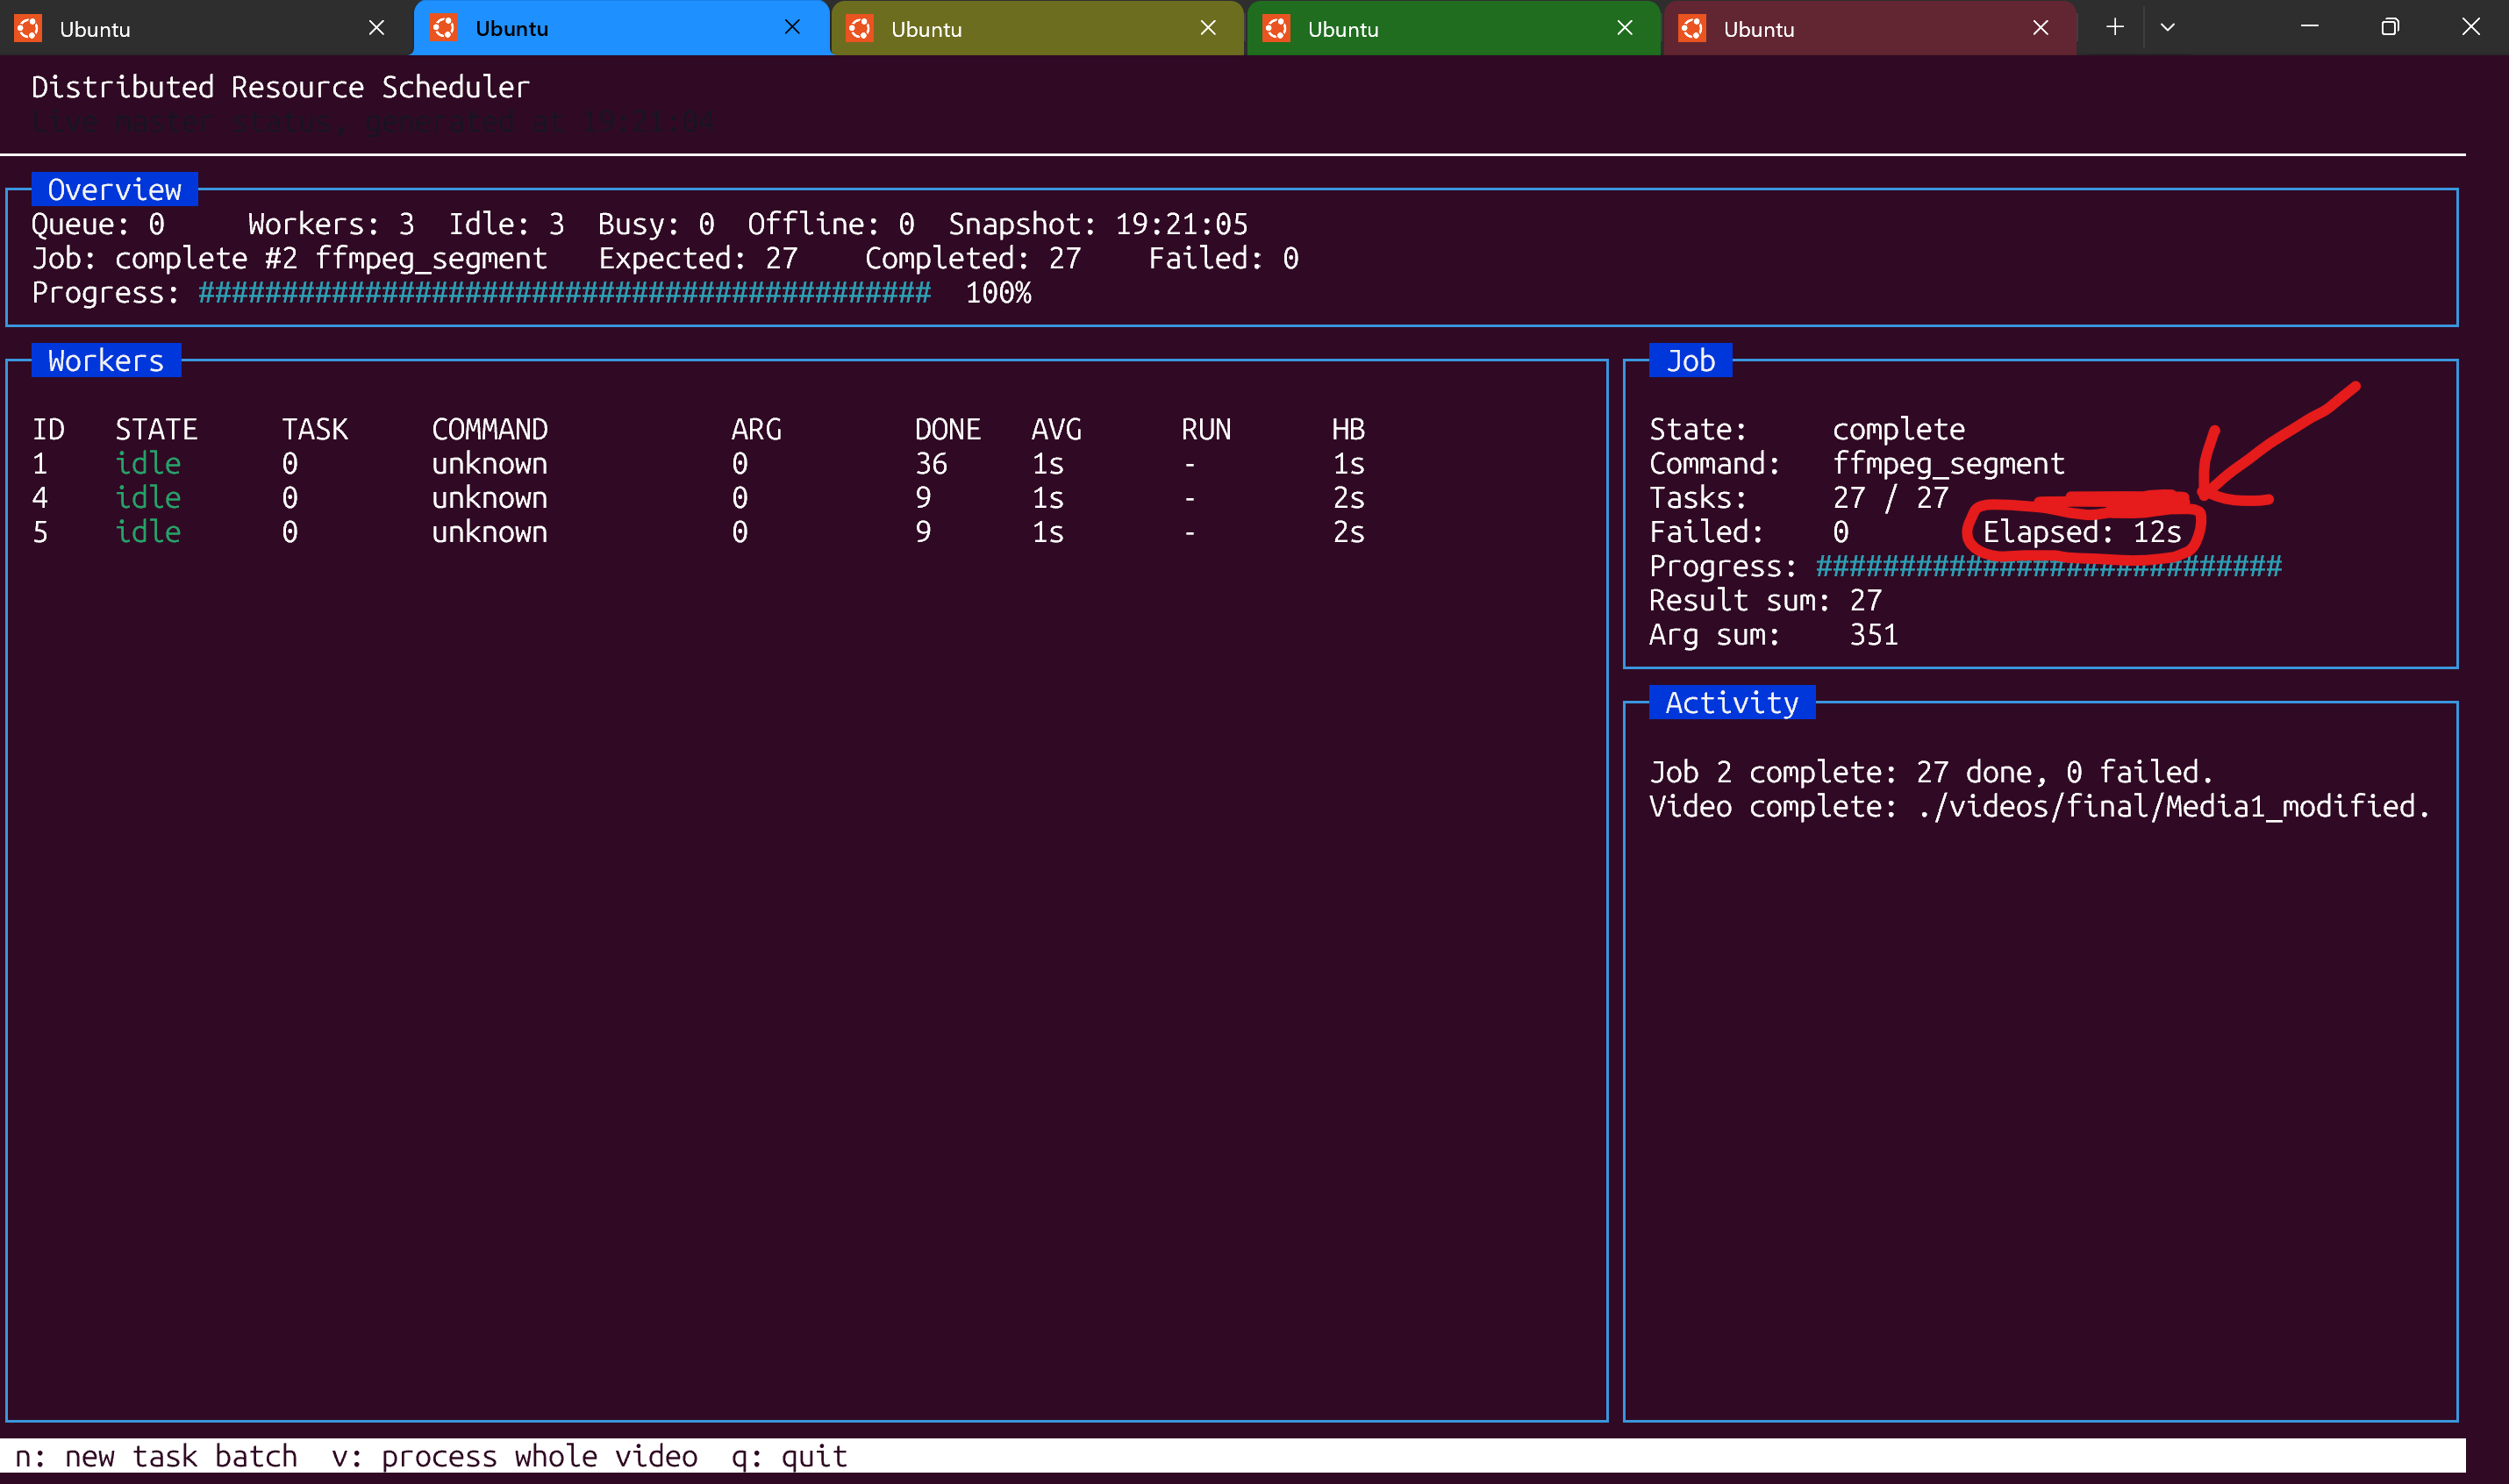
\includegraphics[width=0.95\textwidth]{performance_ffpmeg_using_three_workers.png}
\caption{FFmpeg performance run using three active workers. The elapsed time is lower due to parallel segment processing.}
\end{figure}

\begin{figure}[H]
\centering
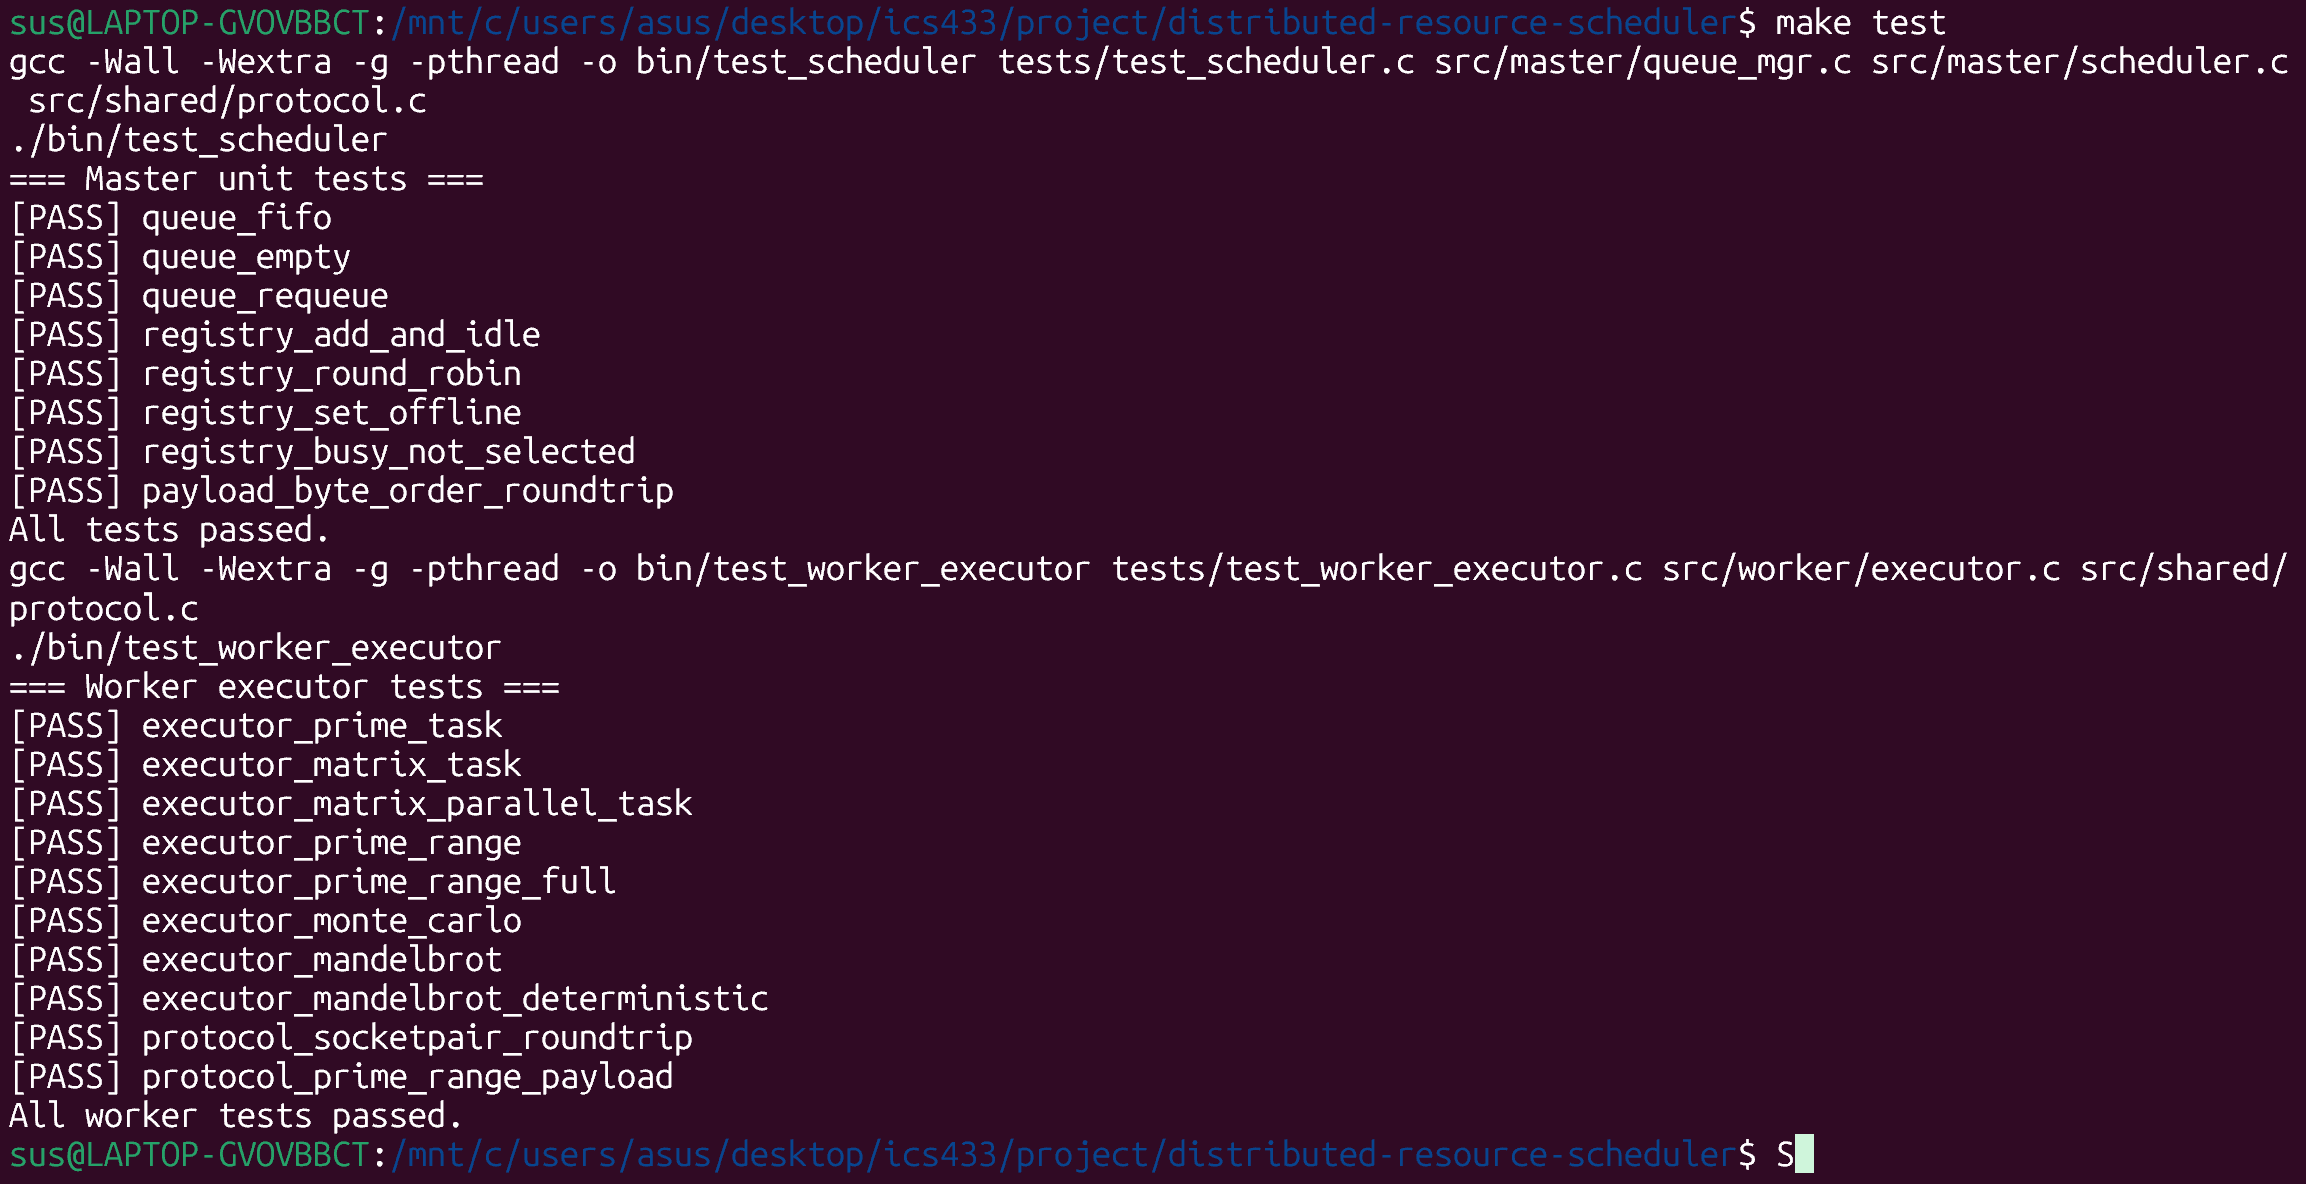
\includegraphics[width=0.95\textwidth]{UnitTestpng.png}
\caption{Unit test output from \texttt{make test}, showing scheduler, queue, registry, protocol, and worker executor tests passing.}
\end{figure}

\subsection{Performance}

The FFmpeg segment workload demonstrates the benefit of parallel execution. In the one-worker screenshot, the dashboard reports an elapsed time of 33 seconds for a 27-segment job. In the three-worker screenshot, the dashboard reports 12 seconds for the same 27-segment workload.

\begin{center}
\begin{tabular}{lccc}
\toprule
\textbf{Configuration} & \textbf{Workers} & \textbf{Elapsed Time} & \textbf{Speedup} \\
\midrule
Single-worker FFmpeg & 1 & 33 s & 1.00x \\
Three-worker FFmpeg & 3 & 12 s & 2.75x \\
\bottomrule
\end{tabular}
\end{center}

The speedup is not exactly 3.00x because of scheduling overhead, worker startup timing, FFmpeg internal threading, video segment size variation, and shared disk I/O. However, the improvement shows that the scheduler successfully distributes independent segment tasks across workers.

\section{Challenges and Solutions}

\subsection{TCP Partial Reads}

TCP is a byte stream, so a single \texttt{recv()} call is not guaranteed to return a full struct. The solution was to implement \texttt{recv\_full()} and \texttt{send\_full()} so every message frame is transmitted completely.

\subsection{Thread Safety and Lock Ordering}

The master has several shared structures, including the queue, registry, and job summary. To avoid deadlock, the implementation avoids holding registry and queue locks at the same time. When a task must be requeued, the task is copied while holding the registry lock, then the lock is released before queue insertion.

\subsection{Worker Disconnect Race}

When a worker disconnects while busy, its current task can be lost if the worker state is cleared too early. The solution was to snapshot the assigned task before marking the worker offline and to keep the last unfinished task visible for dashboard activity reporting.

\subsection{Heartbeat Timeout}

Socket disconnect is not always immediate in real networks. The final implementation adds a scheduler-side timeout: if a worker has not sent a heartbeat for more than 15 seconds, it is marked offline and its unfinished task is requeued.

\subsection{FFmpeg Segment Cleanup}

Processed video segments are needed for merging, but original input segments are not needed after successful processing. The master now deletes each original input segment after receiving a successful FFmpeg result, reducing disk usage during long runs.

\subsection{Dashboard Integration}

The dashboard needed to read live state without blocking scheduler or network threads. The solution was to expose a snapshot API that copies the queue, worker, and job state under locks, then renders the copied state in ncurses.

\section{Future Improvements}

\begin{itemize}[noitemsep]
    \item Add persistent job history so completed job summaries remain visible after new submissions.
    \item Store performance measurements in CSV for graph generation.
    \item Add a configurable heartbeat timeout through environment variables.
    \item Improve FFmpeg task metadata so the dashboard can display video names and segment counts per job.
    \item Add real Raspberry Pi deployment scripts using NFS or Samba shared storage.
    \item Add stronger retry limits so a repeatedly failing task does not loop forever.
    \item Add a web dashboard or JSON API client for easier remote monitoring.
\end{itemize}

\section{Team Contribution}

\begin{center}
\begin{tabular}{p{4cm}p{9cm}}
\toprule
\textbf{Member} & \textbf{Contribution} \\
\midrule
Rayan Alamri & Master server, queue manager, worker registry, scheduler, job summary integration, fault tolerance behavior. \\
Mohammed Alsuhaibani & Worker client, heartbeat thread, executor, task isolation, FFmpeg worker operations. \\
Ali Almuzain & Shared protocol, message model, byte-order conversion, reliable socket send/receive helpers. \\
Mohammed Yar & Terminal dashboard design, activity panel, job panel, worker table, video workflow UI. \\
\bottomrule
\end{tabular}
\end{center}

\section{Code Submission and README}

The final code is organized under the \texttt{src/} directory and built through the root \texttt{Makefile}. The project also includes a detailed \texttt{README.md} and \texttt{MANUAL.md} with requirements, build steps, native execution, Docker execution, FFmpeg pipeline steps, and fault tolerance testing.

\subsection{Requirements}

\begin{itemize}[noitemsep]
    \item Linux, WSL, macOS, or another POSIX-like environment
    \item \texttt{gcc}
    \item \texttt{make}
    \item \texttt{pthread} support
    \item \texttt{ncurses} development package
    \item \texttt{ffmpeg} and \texttt{ffprobe} for video workloads
    \item Docker and Docker Compose for container simulation
\end{itemize}

\subsection{Native Run Commands}

The native run uses separate terminals for the long-running processes. First, build the binaries from the project root:

\begin{lstlisting}[style=shellstyle]
make
\end{lstlisting}

Then start the master in one terminal:

\begin{lstlisting}[style=shellstyle]
./bin/master
\end{lstlisting}

Start each worker in a separate terminal:

\begin{lstlisting}[style=shellstyle]
./bin/worker 127.0.0.1 9090
\end{lstlisting}

Additional workers are launched by repeating the worker command in more terminals. For normal users, task submission is handled through the ncurses dashboard: press \texttt{n} to submit a task batch, or press \texttt{v} to select and process a video.

\subsection{Docker Fixed-Core Simulation}

\begin{lstlisting}[style=shellstyle]
docker build -t drs .
docker network create drs-net

docker run --rm -it --name drs-master \
  --network drs-net \
  -p 9090:9090 \
  -e MASTER_PORT=9090 \
  -e MASTER_DASHBOARD=1 \
  -e TERM=xterm-256color \
  -v "$PWD/videos:/videos" \
  -v "$PWD/logs:/logs" \
  drs master
\end{lstlisting}

Each worker is then launched in a separate terminal:

\begin{lstlisting}[style=shellstyle]
docker run --rm -it --name drs-worker-1 \
  --network drs-net \
  --cpuset-cpus="0,1" \
  -e VIDEO_DIR=/videos \
  -v "$PWD/videos:/videos" \
  -v "$PWD/logs:/logs" \
  drs worker drs-master 9090
\end{lstlisting}

Worker container names cannot be reused while containers are running. If more workers are started, the number in \texttt{--name drs-worker-1} must be changed for each new worker, such as \texttt{drs-worker-2}, \texttt{drs-worker-3}, and so on. If two workers use the same name, Docker will fail because that container name is already in use.

The \texttt{--cpuset-cpus} option pins a worker container to specific host CPU cores. The example uses cores \texttt{0} and \texttt{1}. If the host machine does not have enough CPU cores, the CPU set must be reduced, for example to \texttt{--cpuset-cpus="0"}, or the \texttt{--cpuset-cpus} line can be removed so Docker can schedule the container on any available core.

\section{Conclusion}

The Distributed Resource Scheduler successfully implements a working mini OS-style distributed execution platform. It combines OS-level concurrency, socket communication, scheduling, worker monitoring, fault recovery, and real media-processing workloads. The final system demonstrates that independent jobs can be distributed across workers, that failures can be recovered through requeueing, and that performance improves when parallel workloads such as FFmpeg segment processing are executed by multiple workers.

\end{document}
